\subsection{Convolutional Neural Networks} \label{sec:CNN}
Wie bereits dargestellt, sind alle Neuronen in einem \ac{NN} miteinander verbunden. Dies führt dazu, dass die Zahl der Parameter innerhalb des \ac{NN} schnell steigen kann. Dies ist zum Beispiel bei Bildern, bei denen jeder einzelne Pixel ein eigenen Eingabewert in das Netzwerk darstellt, der Fall. Da für jeden Parameter Berechnungen durchgeführt werden müssen, skalieren \ac{NN} dementsprechend schlecht.

Zusätzlich entstehen Formen und Objekte in Bildern erst durch den räumlichen Zusammenhang einiger Pixel. Daher erscheint das Vorgehen, alle Neuronen im Input Layer (Pixelwerte) mit allen Neuronen im ersten Hidden Layer zu verbinden, als wenig sinnvoll.

Aus diesen und weiteren Gründen, werden heutzutage \ac{CNN} für die Klassifizierung von Bildern verwendet. Durch besondere Bausteine sorgen diese dafür, dass sowohl der räumliche Zusammenhang der Pixel betrachtet wird, als auch die Anzahl von Parametern besser skalierbar ist. Basierend auf den biologischen Vorbildern - siehe nächster Abschnitt - schlugen Fukushima und Miyake im Jahre 1972 \textit{Neocognitron} vor, welches als ein Vorgänger von \ac{CNN} gesehen werden kann.\footcite[Vgl.][S. 267–285]{fukushima1982neocognitron} LeCun et. al verwendeten in ihrem Artikel \textit{Handwritten digit recognition with a back-propagation network} von 1990 einem dem \textit{Convolutional Layer} (siehe Abschnitt \ref{LocalReceptiveFields}) ähnlichen Aufbau.\footcite[Vgl.][S. 396–404]{lecun1990handwritten} Der Artikel \textit{Gradient-based learning applied to document recognition} von LeCun et. al aus dem Jahre 1998 beschreibt das erste Mal den Aufbau eines heute üblichen \ac{CNN}.\footcite[Vgl.][S. 2278–2324]{lecunGradientbasedLearningApplied1998}

\subsubsection{Biologische Grundlagen}
\ac{CNN} basieren auf Beobachtungen der Funktionsweise des visuellen Cortex bei Menschen und Tieren. So haben Hubel und Wiesel 1959 bzw. 1962 gezeigt, das einzelne Sehzellen nur auf Veränderungen in einzelnen Bereichen der Netzhaut reagieren. Dieses Bereiche wurden von Hubel und Wiesel als \textit{receptive field} bezeichnet. \footcite[Vgl. ][S. 574-591]{hubelReceptiveFieldsSingle1959} \footcite[Vgl. ][S. 106-154]{hubelReceptiveFieldsBinocular1962}


\todo{Verweis 13,14 Masterthesis}

\begin{figure}[t]
    \centering
    \caption[]{Vereinfachter Aufbau visueller Cortex und \ac{CNN}}
	\label{fig:humVisVsCNN}
    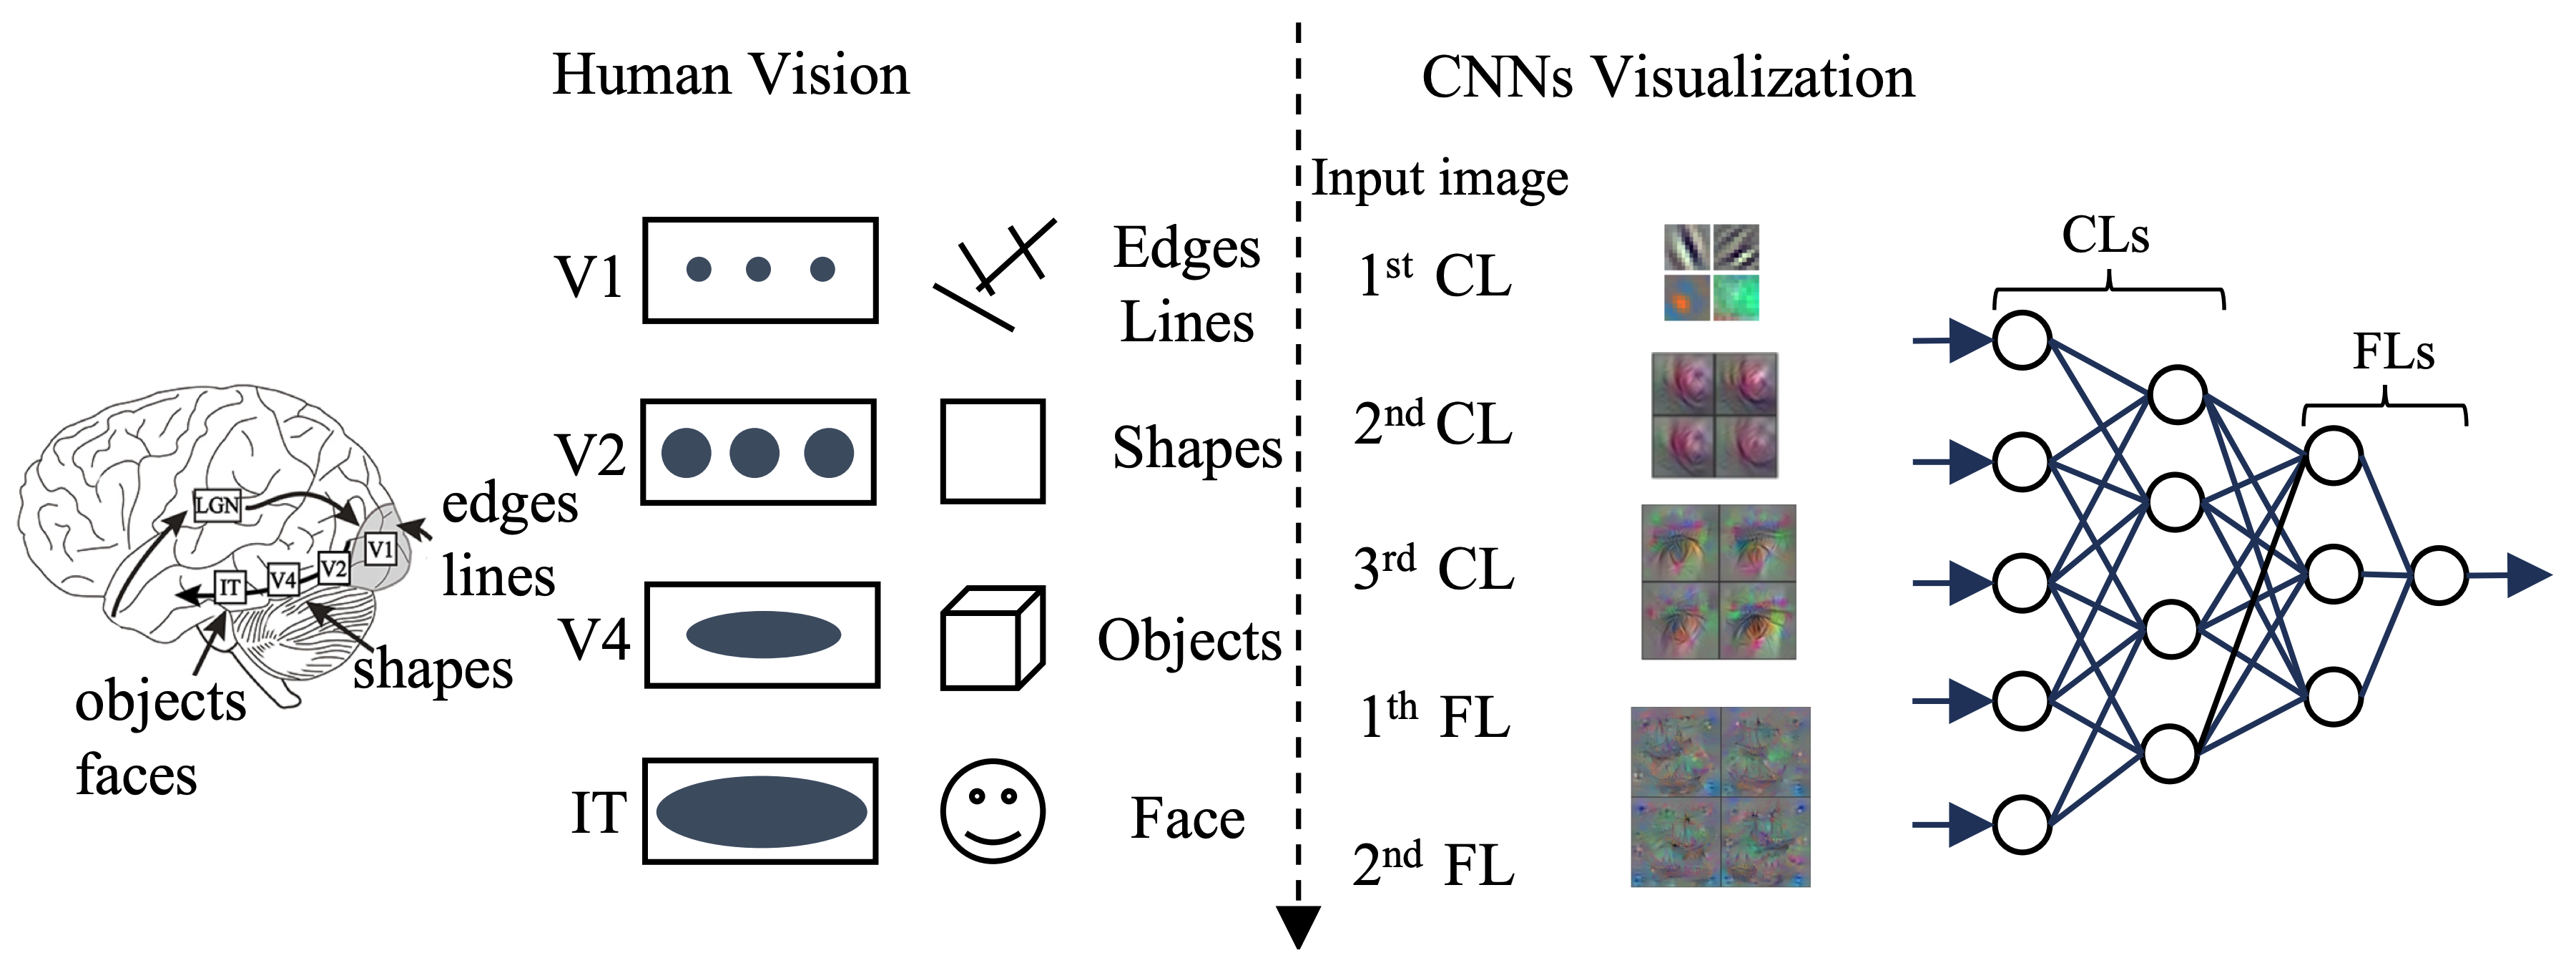
\includegraphics[width=1\textwidth]{human_vis_vs_cnn.png}
    Quelle: Qin et al., 2018
\end{figure}

In Abbildung \ref{fig:humVisVsCNN} wird der vereinfachte visuell Cortex eines Menschen dem Aufbau eines \ac{CNN} gegenübergestellt. Auf der linken Seite ist zu erkennen, dass beim visuellen Cortex verschiedene Schichten (V1, V2, V4 und IT) vorliegen, welche nacheinander geschaltet sind. Jede dieser Schichten enthält \textit{receptive fields}, wobei diese mit jeder Schicht größer werden. Die früheren Schichten reagieren hierbei auf einfache Formen wie Linien oder Kanten und die späteren auf komplexere Formen wie ganze Objekte. Bei allen Schichten können die gesamten Elemente an jeder Stelle des \textit{receptive field} auftreten und trotzdem für eine Aktivierung sorgen. Die rechte Seite zeigt den typischen Aufbau eines \ac{CNN}, bei dem die früheren Schichten (CL) einfache und spätere Schichten (FL) komplexe Formen erkennen. \footcite[Vgl. ][S. 6]{qinHowConvolutionalNeural2018}

\subsubsection{Architektur}
\ac{CNN} haben drei grundlegende Ideen bzw. Bausteine, die sie von anderen \ac{NN} unterscheiden. Diese sind \textit{\ac{LRF}}, \textit{gemeinsame Gewichte und Bias} sowie \textit{Pooling} und werden in diesem Abschnitt genauer beleuchtet.

\paragraph{Local Receptive Fields} \label{LocalReceptiveFields}
Die Grundidee hinter \ac{LRF} ist - ähnlich wie mein visuellen Cortex - Neuronen zu erzeugen, die in bestimmte Bereiche auf Formen reagieren. Anders gesagt, sollen die einzelnen Neuronen einen Teil des Bildes betrachten und hier Formen erkennen können. Stellt man sich das Eingangssignal als Matrix statt einem Vektor vor, lässt sich das ganze einfacher visualisieren. Ein Bild mit 28x28 Pixel entspricht also einer 28x28 Matrix, siehe Abbildung \ref{fig:lrf} links. Um nun die \ac{LRF} nachzubilden, wird eine kleinere Matrix - typischerweise als \textit{Filter} oder \textit{Kernel} bezeichnet - über das Bild geschoben. Typische Maße für den Kernel sind hierbei 3x3, 4x4 oder 5x5. Alle Pixel die vom Kernel übereckt werden, werden in der Berechnung für den Pixelwert in der Ausgabe zusammengefasst (siehe Abbildung \ref{fig:lrf} rechts). Bei einer Matrix mit den Maßen 5x5 bedeutet dies, dass ein Pixel in der Ausgabe 25 Werte zusammenfasst. Die Werte innerhalb der Kernel-Matrix stellen dabei die Gewichte für jeden einzelnen Pixel dar. Zusätzlich hat jeder Pixel in der Ausgabe auch noch einen eigenen Bias.

Wandert der Kernel über das Bild, kann er um \textit{n} Schritte nach rechts bzw. um \textit{m} Schritte nach unten verschoben werden. Hierdurch wird bestimmt, welche Pixel in der Ausgabe zusammengefasst werden. Diese Schrittweite wird als \textit{Stride} bezeichnet. Betrachtet man ein Bild mit 28x28 Pixeln, einen 5x5 Kernel und einen Stride von 1, besteht die Ausgabe aus 24x24 Pixeln. Dies liegt daran, dass man den Kernel von der Ausgangsposition nur 23 Mal um eins nach rechts bzw. unten schieben kann. Um zu verhindern, dass die Matrix im nachfolgendem Layer kleiner wird, kann \textit{Padding} angewendet werden. Hierbei werden um das Bild herum weitere Pixel ergänzt. Typischerweise geschieht dies symmetrisch, allerdings ist es auch möglich unterschiedlich viele Reihen auf jeder Seite hinzuzufügen. Der Wert der hinzugefügten Pixel wird typischerweise auf $0$ gesetzt.

Die Anzahl der Spalten in der Ausgabe kann mit Gleichung \ref{eq:CalcOutputSize} berechnet werden.\footcite[Vgl.][S. 15]{dumoulinGuideConvolutionArithmetic2018} Hierbei steht $i$ für die Anzahl der Spalten in der Matrix die das ursprüngliche Bild darstellt, $p_{links}$ für die Anzahl von Spalten die durch das Padding links hinzugefügt wurden ($p_{rechts}$ dementsprechend für die rechts), $k$ für die Maße des Kernels und $s$ für den Stride. Sind das Bild und der Kernel quadratisch und durch Padding wurde an allen Seiten gleich viele Spalten hinzugefügt, entspricht das Ergebnis auch der Anzahl an Zeilen in der Ausgabe. \footcite[Vgl.][S. 169-171]{nielsenNeuralNetworksDeep2015}

\begin{equation} \label{eq:CalcOutputSize}
    o=\left\lfloor\frac{i+p_{links}+p_{rechts}-k}{s}\right\rfloor+1
\end{equation}


\begin{figure}[t]
    \centering
    \caption[]{Input Layer als Matrix (links) und Beispiel \ac{LRF} zwischen Input und 1. Hidden Layer}
	\label{fig:lrf}
    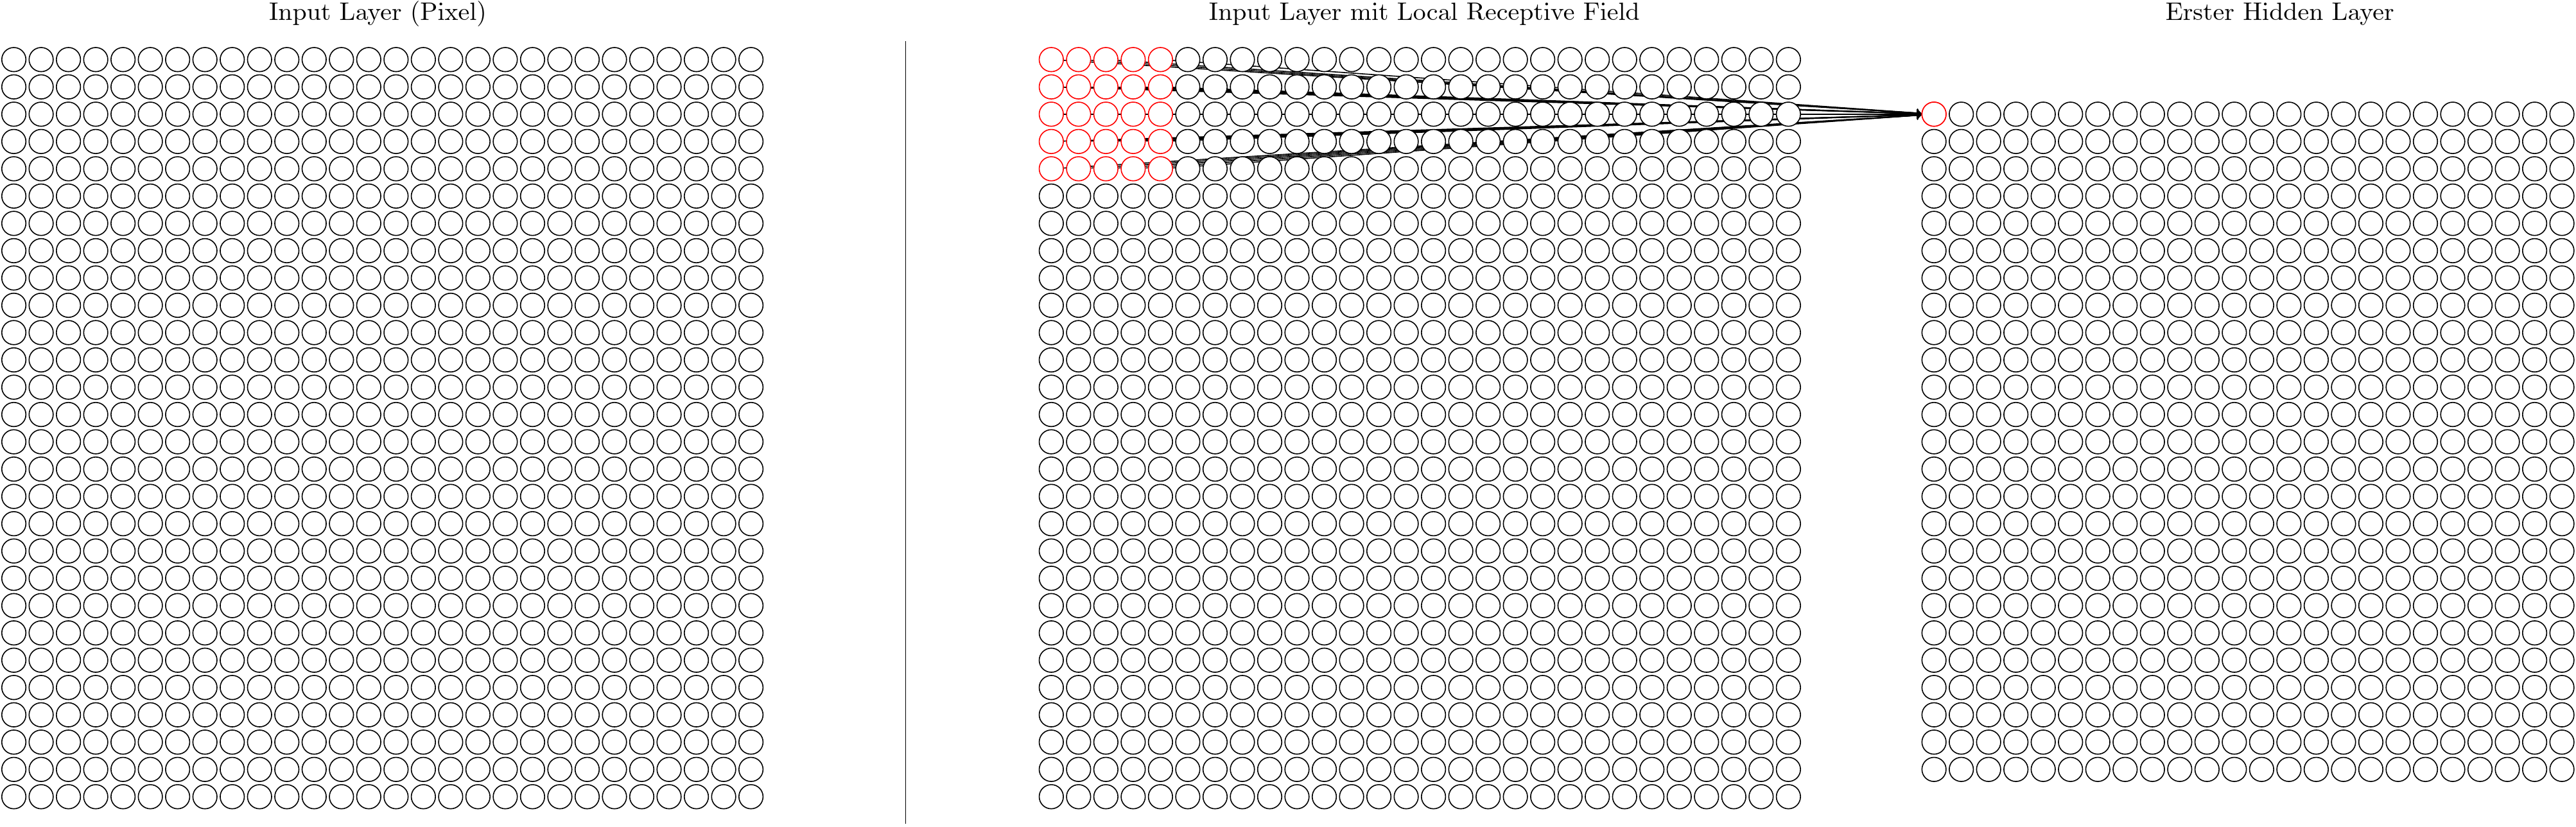
\includegraphics[width=1\textwidth]{lrf.png}
    Quelle: In Anlehnung an Nielsen, Introduction CNN, 2018, S. 170 f.
\end{figure}

\paragraph{Gemeinsame Gewichte und Bias}
Wie bereits erwähnt, stellen die Werte der Kernel-Matrix die Gewichte für jeden einzelnen Pixel im Bild dar. Allerdings werden außerdem die gleichen Werte innerhalb des Kernels für alle Verschiebungen verwendet. Bei einem 28x28 Layer und einer 5x5 Matrix, werden also alle 24x24 Pixel im Ausgang mit den gleichen Gewichten und Bias berechnet (siehe Gleichung \ref{eq:actSharedWeights}).

\begin{equation}
    \label{eq:actSharedWeights}
    pixel_{j,k} = \sigma\left(b+\sum_{l=0}^{z} \sum_{m=0}^{s} w_{l, m} a_{j+l, k+m}\right)
\end{equation}

Hierbei steht ($z$) für die Anzahl der Zeilen und $s$ für die Anzahl von Spalten der Matrix des Bildes. $b$ ist der gemeinsame Bias, $w$ das Gewicht an Position $l,m$ der Matrix und $a$ der Wert innerhalb des Kernels. Typischerweise wird die berechnete Summe noch in eine Aktivierungsfunktion gegeben, welche durch $\sigma$ dargestellt wird.

Das bedeutet, dass durch den Kernel überall auf dem Bild die gleichen Formen beziehungsweise Objekte erkannt werden. Man stelle sich zum Beispiel vor, dass der Kernel durch das Anpassen seiner Gewichte gelernt hat vertikale Linien zu erkennen. Dann ist es sinnvoll, dass diese vertikale Linie überall auf dem Bild erkannt werden kann. Genau dies wird durch die gemeinsamen Gewichte und Bias erreicht.

Das Element, auf welches ein Kernel reagiert, wird als \textit{Feature} bezeichnet. Daher werden die Matrizen in der Ausgabe auch \textit{Feature Maps} genannt. Insgesamt wird ein Layer in einem \ac{CNN}, welcher Feature Maps mit gemeinsamen Gewichten anwendet, als \textit{Convolutional Layer} bezeichnet. Ein \ac{CNN} soll mehr als ein Feature pro Convolutional Layer erkennen können. Daher können pro Convolutional Layer $n$ verschiedene Kernels verwendet werden. Mit jedem Kernel ensteht eine neue Matrix in der Ausgabe. Die Ausgabe stellt somit eine dreidimensionale Matrix dar, bildlich gesehen kann man sich einen Stapel von zweidimensionalen Matrizen vorstellen (siehe Convolution Layer in \ref{fig:convAndPool}).
Grundsätzlich reagieren Kernels in Convolutional Layern die früh im \ac{CNN} vorkommen eher auf einfache Formen wie Kanten oder Ecken. Später reagieren Convolutional Layer dann auf komplexere Formen bzw. Objekte. Auf der rechten Seite in Abbildung \ref{fig:humVisVsCNN} ist dies dargestellt. Währen im ersten CL Layer einfache Linien erkannt werden, kann man im dritten CL Layer bereits Augen erkennen.\footcite[Vgl.][S. 169-171]{nielsenNeuralNetworksDeep2015}

\paragraph{Pooling}
Neben dem beschriebenen Convolutional Layer, haben \ac{CNN} eine weitere besonderen Layer. Dieser wird als \textit{Pooling Layer} bezeichnet und typischerweise direkt hinter einem Convolutional Layer angewendet. 

Ein Pooling Layer vereinfacht hierbei die vorliegenden Informationen, also die Matrizen die der vorherige Layer ausgegeben hat. Folgt der Pooling Layer auf einen Convolutional, sind dies die Ausgaben der Feature Maps, also die Werte, die durch die Berechnung der Aktivierungsfunktion erhalten werden.

Beim Pooling werden mehrere Werte zusammengefasst, es wird also erneut eine Art Filter (Quadrat) über die Matrix gelegt und alle überdeckten Werte werden zusammen betrachtet. Am verbreitesten sind hierbei das \textit{Max Pooling} und das \textit{Average Pooling}. Wie durch die Namen zu erkennen, wird beim Max Pooling der maximale Wert innerhalb der betrachteten Werte verwendet, während beim Average Pooling der Durchschnitt berechnet wird. Beides ist in Abbildung \ref{fig:pooling} beispielhaft dargestellt. Die Maße der Matrix verändern sich entsprechend der gewählten Filter Matrix, bei einer 2x2 Matrix wird die Anzahl der Spalten und Zeilen halbiert.
Das Pooling wird hierbei auf jede Feature Map separat angewendet, die Anzahl der Matrizen ändert sich also nicht. 

Durch Pooling wird geprüft, ob ein Element durch den Convolutional Layer gefunden wurde (= hohe Werte). Die Grundannahme geht hierbei davon aus, dass die Information das dieses Element vorhanden ist, aber nicht die genaue Position relevant ist. Durch das Pooling bleibt die Information erhalten, nur die Genauigkeit der Positionsangabe sinkt. Hierfür wird wiederum die Anzahl der Parameter stark reduziert. 

In Abbildung \ref{fig:convAndPool} ist der Beginn eines \ac{CNN} dargestellt. Hier wird ein Convolutional Layer als erster Hidden Layer verwendet und dessen Ausgabe (Feature Maps) werden als Input für den Pooling Layer (zweiter Hidden Layer) verwendet. Dessen Ausgabe wird in einen Dense Layer gegeben, also einem Layer der mit allen Neuronen des vorherigen Layers verbunden ist.\footcite[Vgl.][S. 169-171]{nielsenNeuralNetworksDeep2015}

\begin{figure}[t]
    \centering
    \begin{tikzpicture}[x=1.5cm, y=1.5cm,  >=stealth]
        \tikzset{square matrix/.style={
            matrix of nodes,
            column sep=-\pgflinewidth, row sep=-\pgflinewidth,
            nodes={draw,
            text height=#1/2+0.75ex,
            text depth=#1/2-0.75ex,
            text width=#1,
            align=center,
            inner sep=0pt
            },
        },
        square matrix/.default=1.4cm
        }

        \matrix[square matrix](matrix)
        {
            |[fill=lightgray]|163 & |[fill=lightgray]|131 &0 & 42   \\
            |[fill=lightgray]|248 & |[fill=lightgray]|247 & 161 & 89  \\
            || 13 & 120 & 62 & 8 \\
            || 40 & 19 & 23 & 168 \\
        };

        \node[text width=6cm] at (5, 1) 
            {\baselineskip=25pt \underline{\textbf{Max Pooling:}} \\ $max(163, 131, 248, 247) = 248$ \par};

        \node[text width=6cm] at (5, -1) 
            {\baselineskip=25pt \underline{\textbf{Average Pooling:}} \\ $\frac{163 + 131 + 248 + 247}{4} = 197$ \par};
        
    \end{tikzpicture}
    \caption[]{Beispiel Max Pooling und Average Pooling}
    \label{fig:pooling}
    Quelle: Eigene Darstellung, 2020
\end{figure}

\begin{figure}[t]
    \centering
    \caption[]{Convolutional und Pooling Layer im Zusammenspiel}
	\label{fig:convAndPool}
    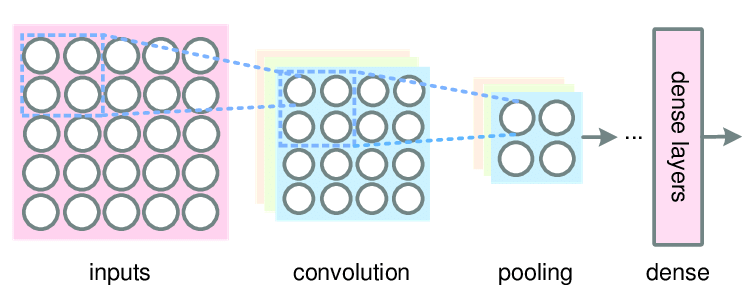
\includegraphics[width=1\textwidth]{overview_cl_pooling.png}
    Quelle: Wang et. al, Wireless Layer, 2017, S. 4
\end{figure}
